\documentclass[11pt,a4paper]{article}

\usepackage[utf8]{inputenc}
\usepackage[T1]{fontenc}
\usepackage[french]{babel}
\usepackage{lmodern}
\usepackage[margin=2.4cm]{geometry}
\usepackage{amsmath,amssymb}
\usepackage{graphicx}
\usepackage{booktabs}
\usepackage{caption}
\usepackage{tikz}
\usetikzlibrary{automata,positioning,arrows}
\usepackage[hidelinks]{hyperref}

\hypersetup{
  pdftitle={Projet 1 DAAR : clone d'egrep},
  pdfauthor={Ramy Sail, Younes Bensallah}
}

\captionsetup{font=small,labelfont=bf}
\graphicspath{{figures/}}

\newcommand{\eps}{\varepsilon}
\newcommand{\motif}[1]{\texttt{#1}}

\title{Projet 1 -- Clone d'\texttt{egrep}\\[2pt]
  \large Recherche de motif par automate et par KMP}
\author{Ramy Sail \and Younes Bensallah}
\date{UE DAAR -- Master 2 -- octobre 2026}

\begin{document}
\maketitle

\section{Introduction}

Le problème est celui de la commande \texttt{egrep} : étant donnés un motif $R$
(une expression régulière) et un fichier texte de $l$ lignes, afficher les lignes
qui contiennent au moins un facteur appartenant au langage de $R$. Comme le
propose le sujet, nous traitons chaque ligne indépendamment, et nous nous limitons
au sous-ensemble suivant de la norme ERE : les lettres, le point (caractère
universel), la concaténation, l'alternative \motif{|}, l'étoile \motif{*} et les
parenthèses. Nous avons ajouté \motif{+}, utilisé dans l'exemple du sujet
\motif{S(a|g|r)+on}. Les autres opérateurs (\motif{?}, \motif{\{\}},
\motif{[]}, \motif{\textasciicircum}, \motif{\$}) sont lus comme des lettres.

Le programme suit les cinq étapes vues en cours :
\begin{enumerate}
  \item motif $\to$ arbre syntaxique (\texttt{RegexParser}) ;
  \item arbre $\to$ automate non déterministe avec $\eps$-transitions, méthode
        d'Aho-Ullman (\texttt{Ndfa}) ;
  \item $\eps$-AFN $\to$ automate déterministe, méthode des sous-ensembles
        (\texttt{Determinisation}) ;
  \item automate déterministe $\to$ automate minimal, algorithme de Moore
        (\texttt{Minimisation}) ;
  \item parcours de chaque ligne par l'automate (\texttt{Dfa}).
\end{enumerate}
Lorsque l'arbre obtenu à l'étape 1 n'est qu'une suite de concaténations de
lettres, le motif est un simple mot : les étapes 2 à 5 sont alors remplacées par
l'algorithme de Knuth-Morris-Pratt (\texttt{Kmp}). Le choix est fait par
\texttt{Recherche.pour}, et l'option \texttt{-{}-dfa} force l'automate pour pouvoir
comparer les deux méthodes. Sans option, la sortie est celle d'\texttt{egrep} (les
lignes trouvées, telles quelles) et le code de retour aussi : 0 si une ligne est
trouvée, 1 sinon, 2 en cas d'erreur. L'option \texttt{-{}-detail} numérote les
lignes et colore les occurrences.

Le code est en Java 21, sans dépendance. Les sections~\ref{sec:arbre}
à~\ref{sec:kmp} décrivent chaque algorithme, la section~\ref{sec:tests} la
manière dont nous avons vérifié les résultats, et la section~\ref{sec:perf} les
performances, comparées à celles de GNU \texttt{grep}.

\section{Du motif à l'arbre syntaxique}
\label{sec:arbre}

\paragraph{Structure de données.} L'arbre (\texttt{RegexTree}) a cinq sortes de
n\oe uds : \texttt{Feuille} (une lettre), \texttt{Point}, \texttt{Concat},
\texttt{Union} et \texttt{Etoile}. Chaque sorte est un \texttt{record} Java qui
porte exactement ses fils, ce qui rend impossible un n\oe ud \texttt{Union} à un
seul fils, par exemple. Les parenthèses ne laissent pas de trace : elles ne font
que modifier la forme de l'arbre.

\paragraph{Algorithme.} En ERE la concaténation est implicite : dans
\motif{ab*}, rien ne sépare \motif{a} de \motif{b*}. Nous commençons donc par
insérer un opérateur de concaténation explicite (un caractère de contrôle, qui ne
peut pas apparaître dans un motif saisi) entre deux éléments qui se suivent.
Le motif est ensuite mis en notation postfixe par l'algorithme
\emph{shunting-yard} de Dijkstra~\cite{dijkstra}, avec les priorités
$\motif{*} = \motif{+} > \text{concaténation} > \motif{|}$. Enfin, une pile
reconstruit l'arbre à partir de la notation postfixe. Les deux passes sont
linéaires en la longueur $m$ du motif. Un motif mal formé (parenthèse non
fermée, opérateur sans opérande) produit une erreur et le code de retour~2.

\paragraph{Remarques.} \motif{e+} est réécrit en \motif{ee*}, ce qui duplique
le sous-arbre $e$. C'est le plus simple, mais l'automate de l'étape 2 grossit
d'autant : pour \motif{(abc)+}, les états de \motif{abc} sont créés deux fois.
Une construction dédiée à \motif{+} (une seule copie et une $\eps$-transition de
retour) éviterait ce doublement. Par ailleurs, nous refusons le motif vide,
\motif{()} et \motif{a||b}, qu'\texttt{egrep} accepte ; ce sont des cas sans
intérêt pratique, mais c'est un écart à la norme.

\section{De l'arbre à l'automate non déterministe}
\label{sec:afn}

\paragraph{Algorithme.} Nous suivons la construction récursive du livre
d'Aho et Ullman~\cite{ahoullman} (chapitre~10), connue aussi sous le nom de
construction de Thompson~\cite{thompson}. Chaque sous-arbre produit un fragment
d'automate qui a un seul état d'entrée et un seul état de sortie, et le n\oe ud
parent recolle les fragments de ses fils :
\begin{itemize}
  \item une lettre $c$ (ou le point) donne deux états reliés par une transition
        étiquetée $c$ (ou par une transition \og joker \fg{}) ;
  \item $e_1e_2$ relie la sortie de $e_1$ à l'entrée de $e_2$ par une
        $\eps$-transition, sans nouvel état ;
  \item $e_1|e_2$ ajoute une entrée qui mène aux deux fragments et une sortie que
        les deux fragments rejoignent ;
  \item $e^*$ ajoute une entrée et une sortie, une $\eps$-transition de l'entrée
        vers la sortie (le mot vide) et une de la sortie de $e$ vers son entrée
        (la répétition).
\end{itemize}

\paragraph{Structure de données et complexité.} Les états sont des entiers ;
pour chacun, l'automate garde la liste de ses transitions étiquetées et la liste
de ses $\eps$-transitions. Chaque feuille et chaque opérateur \motif{|} ou
\motif{*} crée deux états, la concaténation aucun : sans \motif{+}, l'automate a
donc au plus $2m$ états. Chaque état a au plus une transition étiquetée ou deux
$\eps$-transitions sortantes, si bien que le nombre de transitions est aussi
linéaire. La construction se fait en $O(m)$.

\paragraph{Remarque.} Cet automate est petit mais coûteux à simuler : à chaque
caractère lu, il faut suivre tout un ensemble d'états et calculer sa
$\eps$-fermeture, soit $O(m)$ opérations par caractère. C'est ce qui justifie
les étapes 3 et 4.

\section{Déterminisation par la méthode des sous-ensembles}
\label{sec:det}

\paragraph{Algorithme.} La méthode des sous-ensembles (Rabin et
Scott~\cite{rabinscott}) construit un automate déterministe (DFA) dont chaque
état représente un ensemble d'états de l'$\eps$-AFN. L'état initial est
l'$\eps$-fermeture de l'état initial de l'$\eps$-AFN. Pour un état $E$ et un
symbole $c$, la transition mène à l'$\eps$-fermeture des états atteints depuis $E$
en lisant $c$. Un état est final s'il contient l'état final de l'$\eps$-AFN. On
part de l'état initial et on ne crée que les états accessibles, à l'aide d'une
file et d'une table de hachage qui associe à chaque ensemble déjà rencontré son
numéro dans le DFA.

\paragraph{Un alphabet réduit.} Le texte est lu en caractères Java (UTF-16) : un
DFA complet aurait 65\,536 colonnes par état, presque toutes identiques. Or tous
les caractères qui n'apparaissent pas dans le motif se comportent de la même
façon : seules les transitions joker les acceptent. Nous gardons donc une
colonne par lettre du motif, plus une seule colonne \og autre \fg{} pour tous
les autres caractères. L'automate est en outre partiel : l'absence de transition
tient lieu d'état puits. C'est ce qui rend le point utilisable sans énumérer
l'alphabet.

\paragraph{Complexité.} Pour un $\eps$-AFN à $n$ états, le DFA peut avoir
jusqu'à $2^n$ états, et chacun coûte $O(n)$ par symbole à construire. Ce pire cas
est atteint : la section~\ref{sec:etats} le mesure sur une famille de motifs dont
le DFA a $2^{k+1}$ états. Sur des motifs courants en revanche, l'explosion ne
se produit pas : pour les huit motifs de la section~\ref{sec:perf}, la
construction complète (étapes 1 à 4) prend entre 0,08 et 1~ms.

\section{Minimisation}
\label{sec:min}

\paragraph{Algorithme.} Nous utilisons l'algorithme de Moore~\cite{moore}, par
raffinement de partition. On part de deux classes, les états finaux et les
autres. À chaque tour, deux états restent dans la même classe s'ils y étaient
déjà et si, pour chaque symbole, leurs successeurs sont dans la même classe.
Concrètement, chaque état reçoit une \og signature \fg{} (sa classe, puis la
classe de son successeur pour chaque colonne), et les états de même signature
forment la nouvelle classe. On s'arrête quand le nombre de classes ne change
plus. Comme notre DFA est partiel, nous ajoutons l'état puits pendant le
calcul, puis nous retirons sa classe, qui contient aussi les éventuels états
morts. L'automate minimal est reconstruit avec un représentant par classe.

\paragraph{Complexité et littérature.} Chaque tour coûte $O(n\,|\Sigma|)$ et il
y a au plus $n$ tours, d'où $O(n^2|\Sigma|)$ dans le pire cas. L'algorithme de
Hopcroft~\cite{hopcroft} atteint $O(|\Sigma|\, n \log n)$ en ne raffinant que
par rapport à la plus petite des deux moitiés d'une classe coupée. Nous avons
gardé Moore, plus simple, car la minimisation ne coûte presque rien ici : sur
nos motifs, les étapes 1 à 4 réunies prennent au plus 1~ms.

\paragraph{Apport réel.} La minimisation est garantie optimale, mais elle gagne
peu sur nos motifs. Pour \motif{S(a|g|r)+on}, l'automate minimal a cinq états
(figure~\ref{fig:figure1}), et sur la famille de la section~\ref{sec:etats} elle
ne retire qu'un état sur $2^{k+1}+1$. Elle reste utile quand le motif contient
des redondances, par exemple \motif{a|a} ou \motif{(a*b*)*}, et elle nous a servi
de vérification : un automate minimal est unique, ce qui donne un point de
comparaison fiable dans les tests.

\begin{figure}[ht]
\centering
\begin{tikzpicture}[shorten >=1pt, node distance=2.1cm, on grid, auto, >=stealth,
    every state/.style={minimum size=7mm, inner sep=1pt}]
  \node[state, initial, initial text=] (q0) {$q_0$};
  \node[state] (q1) [right=of q0] {$q_1$};
  \node[state] (q2) [right=of q1] {$q_2$};
  \node[state] (q3) [right=of q2] {$q_3$};
  \node[state, accepting] (q4) [right=of q3] {$q_4$};
  \path[->]
    (q0) edge node {\texttt{S}} (q1)
    (q1) edge node {\texttt{a,g,r}} (q2)
    (q2) edge [loop above] node {\texttt{a,g,r}} ()
    (q2) edge node {\texttt{o}} (q3)
    (q3) edge node {\texttt{n}} (q4);
\end{tikzpicture}
\caption{Automate minimal de \motif{S(a|g|r)+on}, produit par le programme. Les
transitions absentes mènent à l'état puits, qui n'est pas représenté.}
\label{fig:figure1}
\end{figure}

\section{Recherche dans une ligne}
\label{sec:recherche}

\paragraph{Le problème.} L'automate reconnaît les mots du langage de $R$, alors
qu'il faut savoir si une ligne en \emph{contient} un. La méthode vue en cours
lance l'automate depuis chaque position de la ligne, ce qui coûte $O(n^2)$ pour
une ligne de $n$ caractères dans le pire cas.

\paragraph{Notre choix.} Nous construisons l'automate de $\motif{.*}R$ plutôt
que celui de $R$. Une ligne contient un facteur reconnu par $R$ si et seulement
si l'un de ses préfixes est reconnu par $\motif{.*}R$. Il suffit donc d'un seul
parcours de la ligne, arrêté au premier état final rencontré : la recherche
devient linéaire, $O(n)$ par ligne. L'arbre de $\motif{.*}R$ est construit
directement, sans repasser par le texte du motif, et suit ensuite les étapes 2 à
4 comme les autres.

\paragraph{Le prix à payer.} L'automate de $\motif{.*}R$ peut être beaucoup plus
gros que celui de $R$, car il doit se souvenir de toutes les occurrences
commencées en même temps. Pour $R = \motif{a(a|b)}^k$, l'automate minimal de $R$
est une simple chaîne de $k+2$ états, alors que celui de $\motif{.*}R$ en a
$2^{k+1}$ : il doit retenir lesquels des $k+1$ derniers caractères étaient des
\motif{a}. C'est la famille mesurée à la section~\ref{sec:etats}. Pour les motifs
d'un utilisateur d'\texttt{egrep}, ce cas est rare, et le gain linéaire l'emporte.

\paragraph{Repérage des occurrences.} L'option \texttt{-{}-detail} doit en plus
colorer chaque occurrence, ce qui demande ses bornes. Nous utilisons alors un
second automate, celui de $R$ seul, que nous lançons à chaque position jusqu'à
trouver une occurrence, en gardant la plus longue, puis nous reprenons après sa
fin, comme \texttt{egrep -{}-color}. Ce calcul est quadratique dans le pire cas,
mais il n'est fait que sur les lignes déjà retenues, et seulement avec
\texttt{-{}-detail}.

\section{Le cas d'un mot : Knuth-Morris-Pratt}
\label{sec:kmp}

\paragraph{Problème et algorithme.} Quand le motif est un mot $F$ de longueur
$m$, la recherche revient à trouver un facteur dans une chaîne. L'algorithme
naïf compare $F$ à chaque position et recule dans le texte après un échec, d'où
$O(nm)$. L'algorithme de Knuth, Morris et Pratt~\cite{kmp} ne recule jamais dans
le texte : quand le caractère $F[j]$ ne correspond pas, une table de report
indique à quel indice de $F$ reprendre la comparaison. $\mathit{report}[j]$ est
la longueur du plus long bord propre de $F[0..j-1]$ (un préfixe qui est aussi un
suffixe), et vaut $-1$ quand il faut avancer d'un caractère dans le texte. Comme
dans le cours, nous utilisons la version améliorée de la table : si
$F[\mathit{report}[j]] = F[j]$, reprendre à $\mathit{report}[j]$ échouerait sur le
même caractère, on prend donc directement $\mathit{report}[\mathit{report}[j]]$.
Nos tables sont celles du cours, par exemple $[-1, 0, -1, 1, 0]$ pour
\motif{mami} et $[-1, 0, 0, -1, 0, 2, 0]$ pour \motif{chicha}.

\paragraph{Complexité.} Le calcul de la table coûte $O(m)$ et la recherche
$O(n)$ : à chaque caractère du texte, l'indice $j$ augmente au plus de un, et
chaque report le fait diminuer, donc le nombre total de reports est borné par
$n$. La structure de données se réduit au tableau des caractères de $F$ et au
tableau $\mathit{report}$.

\paragraph{Critique.} KMP a la même complexité que notre automate de
$\motif{.*}R$ (qui est d'ailleurs, pour un mot, essentiellement l'automate des
occurrences de $F$), mais il n'a rien à construire et il compare des caractères
dans un tableau au lieu de consulter une table de transitions. En pratique, il
est trois fois plus rapide que notre automate (section~\ref{sec:perf}). Il n'est
pas pour autant optimal : l'algorithme de Boyer-Moore~\cite{boyermoore} compare
le mot en partant de sa fin et peut sauter jusqu'à $m$ caractères d'un coup. Il
est sous-linéaire en moyenne sur un texte en langue naturelle, et c'est lui
qu'utilise GNU \texttt{grep} pour les mots~\cite{haertel}. L'avantage de KMP est
de lire chaque caractère une seule fois et dans l'ordre, ce qui convient à un
flux qu'on ne peut pas relire.

\section{Tests}
\label{sec:tests}

\paragraph{Instances.} Comme le recommande le sujet, nos textes viennent du
projet Gutenberg : six livres de tailles et de styles différents, dont le texte
de la figure~1 du sujet (\textit{A History of Babylon}, 763~Ko), \textit{Alice},
\textit{Sherlock Holmes}, \textit{Moby Dick}, \textit{Guerre et Paix} (3,4~Mo) et
\textit{Candide}, en français, pour les caractères accentués. Ils sont gardés
tels que Gutenberg les distribue, en UTF-8 avec des fins de ligne CRLF. Le corpus
fait 6,4~Mo et 121\,817 lignes. Pour les mesures selon la taille, il est recopié
jusqu'à 32~Mo.

\paragraph{Tests unitaires.} 60 tests JUnit couvrent chaque étape. Les plus
utiles comparent deux implémentations indépendantes sur \emph{toutes} les entrées
courtes : l'$\eps$-AFN simulé directement, le DFA et le DFA minimal doivent
accepter exactement les mêmes mots parmi les 1\,365 mots de longueur au plus 5
sur l'alphabet $\{a, b, c, x\}$ ($x$ n'apparaît dans aucun motif et teste la
colonne \og autre \fg{}) ; KMP doit donner le même résultat que
\texttt{String.contains}, puis que l'automate, sur tous les mots de longueur au
plus 8 sur $\{a, b\}$. D'autres tests vérifient les tables de report du cours,
les cinq états de l'automate minimal de \motif{S(a|g|r)+on}, et le fait que
minimiser un automate déjà minimal ne change rien.

\paragraph{Comparaison avec \texttt{egrep}.} Le sujet demande le même résultat
qu'\texttt{egrep}. Notre banc d'essai le vérifie à chaque exécution : pour chacun
des huit motifs de la section~\ref{sec:perf}, la sortie du clone est comparée
octet par octet à celle de GNU \texttt{grep -E} sur tout le corpus, et KMP et
l'automate doivent trouver les mêmes lignes. Un écart avec \texttt{egrep} est
apparu en cours de projet, sur les fins de ligne : nous lisions d'abord le
fichier avec \texttt{BufferedReader.readLine}, qui coupe aussi sur
\texttt{\textbackslash r}. Or
\texttt{egrep} ne coupe que sur \texttt{\textbackslash n} et garde le
\texttt{\textbackslash r} dans la ligne, où le point peut le reconnaître. Nous
coupons désormais le fichier sur l'octet \texttt{\textbackslash n}, qui ne peut
pas apparaître au milieu d'un caractère UTF-8, avant de décoder chaque ligne.
Dans les conditions de mesure (\texttt{LC\_ALL=C.UTF-8}), les sorties sont
identiques pour les huit motifs.

\section{Performances}
\label{sec:perf}

\paragraph{Protocole.} Les mesures ont été faites sur un Intel Core i7-1360P,
sous Linux (WSL2), avec Java 21 et GNU \texttt{grep} 3.11. Chaque mesure est
répétée 10 fois après 3 exécutions à vide, qui laissent le compilateur à la volée
de Java optimiser le code ; nous donnons la moyenne et l'écart type, représenté
par les barres d'erreur. Nous mesurons à deux niveaux :
\begin{itemize}
  \item \emph{recherche seule} : l'appel de la recherche sur chaque ligne, les
        lignes étant déjà en mémoire. C'est le coût de l'algorithme ;
  \item \emph{commande complète} : \texttt{java -jar egrep.jar} ou
        \texttt{egrep}, lancés comme dans un terminal. C'est ce que voit
        l'utilisateur, et c'est la seule façon de comparer le clone à
        \texttt{egrep}.
\end{itemize}
La sortie des commandes est écrite dans un fichier et non dans
\texttt{/dev/null} : GNU \texttt{grep} détecte \texttt{/dev/null} et s'arrête à
la première ligne trouvée, ce qui faussait nos premières mesures (1~ms au lieu
de 18).

\subsection{Selon la taille du texte}

La figure~\ref{fig:taille} montre que tous les temps sont linéaires en la taille
du texte, ce qu'annonce l'analyse. Pour la recherche seule, KMP traite environ
3,5~ms par Mo et l'automate 12,4~ms par Mo sur le mot \motif{Babylon}. Le motif
\motif{S(a|g|r)+on} coûte autant que \motif{Babylon} avec l'automate, car le DFA
fait une transition par caractère quel que soit le motif : une fois l'automate
construit, la complexité du motif ne compte plus.

\begin{figure}[ht]
\centering
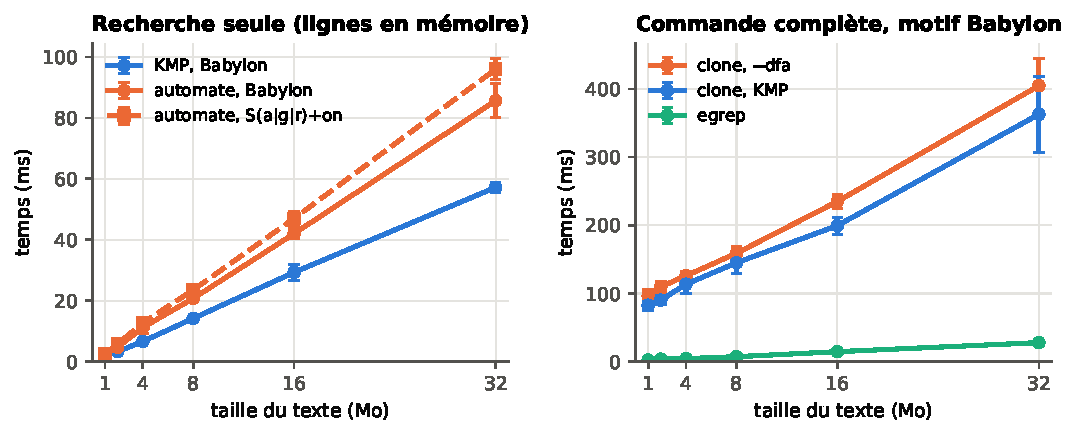
\includegraphics[width=\textwidth]{taille}
\caption{Temps de recherche selon la taille du texte (corpus recopié de 1 à
32~Mo). À gauche, la recherche seule ; à droite, la commande complète, démarrage
de Java compris.}
\label{fig:taille}
\end{figure}

Pourquoi l'automate est-il 3,5 fois plus lent que KMP, alors que les deux
lisent chaque caractère une fois ? Notre table de transitions est une
\texttt{HashMap<Character, Integer>} par état : chaque caractère lu coûte un
calcul de hachage et une indirection, contre une simple comparaison de deux
caractères pour KMP, qui reporte rarement sur un texte en langue naturelle.
Remplacer cette table par un tableau d'entiers indexé par l'état et par la
colonne du caractère est la première amélioration à faire (section~\ref{sec:conclusion}).

\subsection{Selon le motif}

La figure~\ref{fig:motifs} donne le temps de huit motifs sur tout le corpus :
trois mots plus ou moins fréquents, puis un exemple pour chaque opérateur. Pour
la recherche seule, le mot fréquent \motif{the} est le plus rapide avec les deux
méthodes : il apparaît dans 46\,\% des lignes, et la recherche s'arrête à la
première occurrence au lieu de lire la ligne entière. À l'inverse, \motif{Babylon}
est rare et oblige à lire presque toutes les lignes jusqu'au bout. KMP est 2,3 à
3,5 fois plus rapide que l'automate sur les trois mots.

\begin{figure}[ht]
\centering
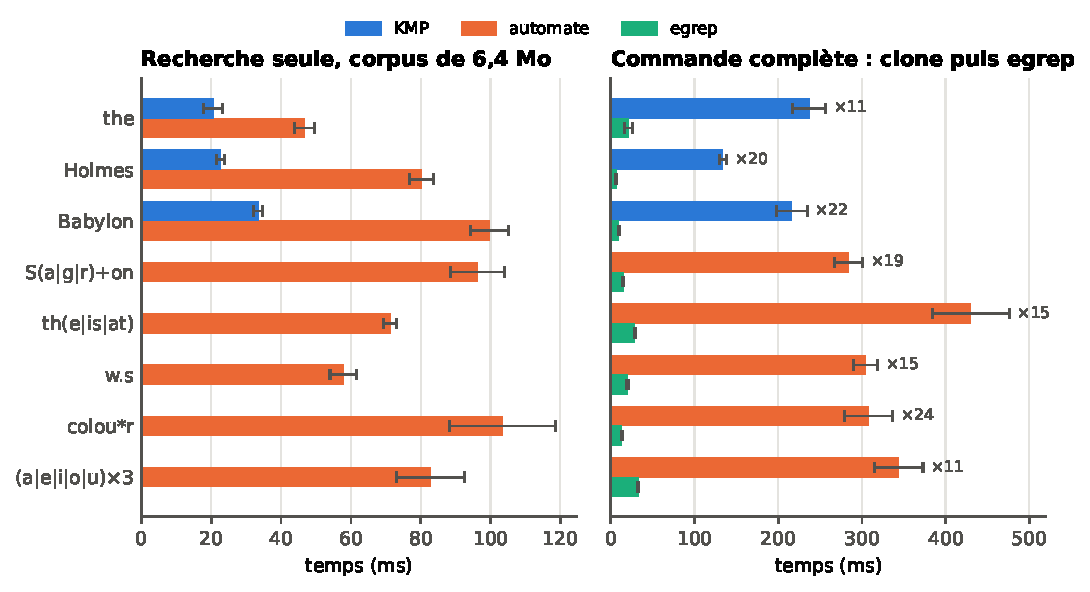
\includegraphics[width=\textwidth]{motifs}
\caption{Temps par motif sur le corpus complet (6,4~Mo). À gauche, la recherche
seule ; pour les trois mots, KMP et l'automate. À droite, la commande complète
du clone (avec la méthode qu'il choisit) et celle d'\texttt{egrep} ; le facteur
indique combien de fois le clone est plus lent.}
\label{fig:motifs}
\end{figure}

\subsection{Comparaison avec \texttt{egrep}}

En commande complète, le clone est 11 à 24 fois plus lent qu'\texttt{egrep}
(figure~\ref{fig:motifs}, à droite). Une partie de l'écart est fixe : sur un
fichier vide, le clone met 54~ms (écart type 6,6) à s'exécuter, contre 1,4~ms
pour \texttt{egrep}, et c'est presque entièrement le démarrage de la machine
virtuelle Java. Le reste grandit avec le texte : à 32~Mo, la commande complète
avec KMP prend 316~ms alors que la recherche seule n'en prend que 111. La
différence correspond à ce que le clone fait en plus de chercher : lire le
fichier entier, le découper, décoder chaque ligne en chaîne Java, écrire les
lignes trouvées, le tout au début avec du code que le compilateur à la volée n'a
pas encore optimisé. Le nombre de lignes écrites compte aussi : avec KMP,
\motif{the} et \motif{Holmes} ont le même temps de recherche, mais la commande
complète coûte 100~ms de plus pour \motif{the}, qui fait écrire 56\,018 lignes
au lieu de 460.

GNU \texttt{grep} évite presque tous ces coûts~\cite{haertel} : il travaille sur
les octets sans les décoder, lit le fichier par blocs, cherche le motif dans le
bloc entier et ne délimite la ligne qu'autour d'une occurrence trouvée. Pour un
mot, il utilise Boyer-Moore, qui ne regarde qu'une partie des caractères ; pour
une expression régulière, il construit l'automate déterministe à la demande,
seulement pour les états réellement atteints. Enfin, les commandes complètes sont
nettement plus dispersées que la recherche seule (écart type jusqu'à 134~ms pour
\motif{Babylon} avec l'automate), ce que nous attribuons au système de fichiers
de WSL2 et à la variabilité du démarrage de Java.

\subsection{Explosion du nombre d'états}
\label{sec:etats}

La figure~\ref{fig:etats} mesure le pire cas de la méthode des sous-ensembles,
sur $\motif{a(a|b)}^k$ recherché dans une ligne (donc l'automate de
$\motif{.*a(a|b)}^k$), pour $k$ de 1 à 12. L'$\eps$-AFN grandit linéairement
($6k+6$ états, soit 78 pour $k = 12$), alors que le DFA en a $2^{k+1}+1$ et le
DFA minimal $2^{k+1}$ : la minimisation ne peut rien fusionner, puisque ces états
correspondent à des contenus différents des $k+1$ derniers caractères. Le temps de
construction suit, et double à peu près à chaque $k$ : 121~ms pour 8\,192 états.
C'est le risque de la déterminisation complète, et la raison pour laquelle les
outils réels la font à la demande.

\begin{figure}[ht]
\centering
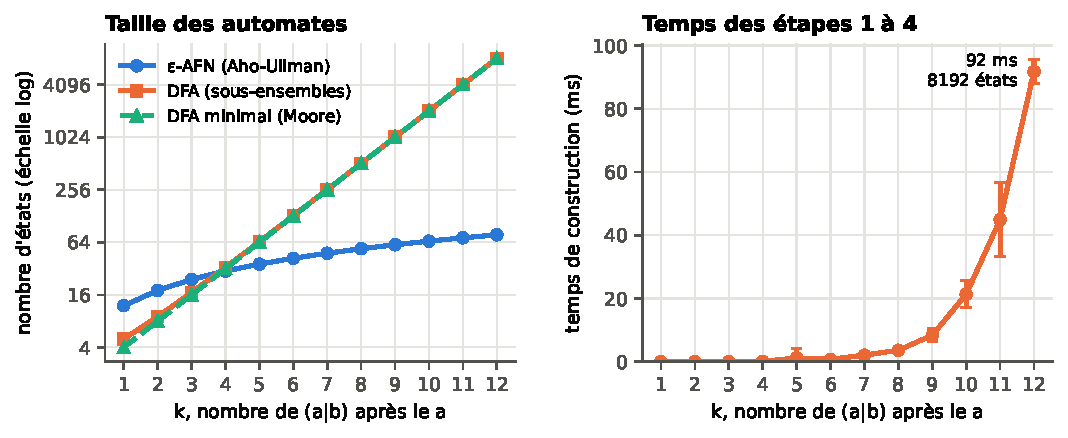
\includegraphics[width=\textwidth]{etats}
\caption{Motif $\motif{a(a|b)}^k$ : nombre d'états des trois automates (échelle
logarithmique) et temps de construction des étapes 1 à 4.}
\label{fig:etats}
\end{figure}

\section{Conclusion et perspectives}
\label{sec:conclusion}

Notre clone implémente les cinq étapes du cours et KMP, et il donne exactement la
sortie d'\texttt{egrep} sur nos instances. La recherche est linéaire grâce à
l'automate de $\motif{.*}R$, au prix d'un automate qui peut devenir exponentiel
sur des motifs construits pour cela. Les mesures montrent que la complexité
asymptotique ne suffit pas à expliquer les temps : à complexité égale, KMP est
trois fois plus rapide que l'automate, et le clone reste plus de dix fois plus
lent qu'\texttt{egrep}, surtout à cause de ce qui entoure la recherche.

Plusieurs améliorations sont possibles, dans l'ordre de leur rapport
gain/effort :
\begin{itemize}
  \item \textbf{une table de transitions en tableau} \texttt{int[][]}, avec un
        petit tableau qui associe à chaque caractère sa colonne : c'est la cause
        identifiée de l'écart entre l'automate et KMP ;
  \item \textbf{chercher sur les octets} plutôt que sur des chaînes décodées, et
        ne délimiter les lignes qu'autour des occurrences, comme \texttt{grep} ;
  \item \textbf{Boyer-Moore} à la place de KMP pour les mots, et, pour une
        expression régulière, chercher d'abord avec Boyer-Moore un mot que toute
        occurrence doit contenir (\motif{on} dans \motif{S(a|g|r)+on}) avant
        de lancer l'automate ;
  \item \textbf{une déterminisation à la demande}, qui ne crée un état du DFA
        que lorsqu'il est atteint par le texte et supprime l'explosion de la
        section~\ref{sec:etats} dans la pratique~\cite{cox}.
\end{itemize}
Enfin, si l'on cherche souvent dans les mêmes textes, comme un moteur de
recherche hors ligne, il vaut mieux payer une fois un précalcul : une table
d'index de tous les mots du texte, consultée par une table de hachage, un arbre
de préfixes (\emph{P-trie}) ou un filtre de Bloom. La recherche d'un mot ne
dépend alors plus de la taille du texte. Pour une expression régulière, on peut
lancer l'automate sur la liste des mots de l'index, bien plus courte que le
texte, au lieu du texte entier.

\section*{Usage de l'intelligence artificielle}

Dans le cadre de ce projet, nous avons utilisé Claude afin de générer les mesures ainsi que les scripts produisant
les figures. Egalement pour l'implémentation de l'algorithme KMP.

\begin{thebibliography}{9}
\small
\bibitem{ahoullman} A.~V. Aho, J.~D. Ullman. \emph{Foundations of Computer
  Science}, chapitre~10, \og Patterns, Automata, and Regular Expressions \fg{}.
  Computer Science Press, 1992.
\bibitem{boyermoore} R.~S. Boyer, J.~S. Moore. A fast string searching
  algorithm. \emph{Communications of the ACM}, 20(10), p.~762--772, 1977.
\bibitem{cox} R.~Cox. Regular expression matching can be simple and fast.
  \url{https://swtch.com/~rsc/regexp/regexp1.html}, 2007.
\bibitem{dijkstra} E.~W. Dijkstra. Algol 60 translation. Rapport MR~34/61,
  Mathematisch Centrum, Amsterdam, 1961.
\bibitem{haertel} M.~Haertel. Why GNU grep is fast. Liste de diffusion
  \texttt{freebsd-current}, 2010.
\bibitem{hopcroft} J.~E. Hopcroft. An $n \log n$ algorithm for minimizing states
  in a finite automaton. \emph{Theory of Machines and Computations}, Academic
  Press, 1971.
\bibitem{kmp} D.~E. Knuth, J.~H. Morris, V.~R. Pratt. Fast pattern matching in
  strings. \emph{SIAM Journal on Computing}, 6(2), p.~323--350, 1977.
\bibitem{moore} E.~F. Moore. Gedanken-experiments on sequential machines.
  \emph{Automata Studies}, Princeton University Press, 1956.
\bibitem{rabinscott} M.~O. Rabin, D.~Scott. Finite automata and their decision
  problems. \emph{IBM Journal of Research and Development}, 3(2), p.~114--125, 1959.
\bibitem{thompson} K.~Thompson. Regular expression search algorithm.
  \emph{Communications of the ACM}, 11(6), p.~419--422, 1968.
\end{thebibliography}

\end{document}
